\chapter{神经信号压缩}

在植入式脑机接口(invasive Brain Machine Interface)中,我们将多电极阵列(multi-electrode array, MEA)植入大脑皮层从而获取高质量的电神经信号。 这种信号的采样率为30kHz, 给数据存储和传输带来了重大负荷, 所以我们需要对数据进行压缩来降低数据量。在这一节中,我们结合大脑运动皮层神经电信号的特性,提出了一种高保真压缩算法。实验中,我们将该算法应用于哺乳动物的大脑运动皮层信号,相对原信号得到了18\%的压缩率,而且没有对信号重建产生明显影响。该方法的信噪比(signal to noise ratio, SNR)达到36dB,而且spike信号也保存下来92\%,大幅超过已有工作的效果。 本章工作发表在IJCNN 2014\cite{}.

\section{神经电信号(electroneurographic signal)}

本章中我们将主要关注运动皮层神经信号。作为大脑皮层的一个重要部分,运动皮层负责计划,控制并执行人体主动行为。在运动皮层功能的相关研究中,电极阵列所采集的多通道信号通常在每个通道进行分频。通道中信号低频部分(截止频率在100Hz)对应神经信号的局部场电位(local field potential, LFP),而中频到高频部分对应于动作电位(spikes)。LFP主要源于前突触行为,反映了很多树突行为的平均电流。与之相反,Spike主要反映兴奋神经元的行为。LFP和spike信号对神经解码都很重要。对于运动皮层而言,spike通常的持续时间小于1毫秒,因此需要用高分辨率设备进行信号采集。这里我们用多电极阵列刺入细胞去采集数以百计的感兴趣神经元的信号。哺乳动物运动皮层神经元信号通常以20-30kHz的频率采集128个通道,以保证可以完好保存spike细节。这样,以16-bit的A/D分辨率计算,如果采样率为30kHz,那么128个通道的信号就会以7.68MB/s的速度进行采集。换句话说,一小时内的信号量就积累到28.8GB,这对信号的存储和传输都带来了巨大挑战。所以,我们要对信号进行压缩。

尽管BMI系统已经建立得比较完善了,脑皮层胞外信号的记录并没有深入研究过。在Electromyography(EMG)和Electroencephalography(EEG)信号的压缩上有过一些相关工作\cite{},为了有效压缩,他们都结合了所处理信号的信号特性。但是植入式胞外信号与之相差甚远。

现有多通道压缩算法从两种思路进行实现。一种是应用通道内特性对每个通道的信号分别进行压缩,另一种是用通道间相关性同时对所有通道的信号进行压缩。从第一个思路出发,Weber等人通过基于小波的编码器对老鼠躯体感觉皮质(S1区)进行压缩,然后这种方法代价是丢掉了25\%的spike,对于后期的信号还原和分析并不理想。Chen等人对老鼠的S1区域进行研究,通过自适应信号量化在信噪比保持25db的时候达到的压缩率高于25\%,那么信号压缩率和信号质量都得不到保证。为了改善他们的工作,Chen从第二种思路出发,利用通道间的信号相关性,在25db信噪比的情况下,将压缩率降至5\%。然而,以上几种方法都丢失了太多信号细节,白费了采集来的高分辨率信号。

本章中,我们提出了一个运动皮层胞外信号的高保真压缩框架。 首先,我们讨论这种信号的3个特性:1) 信号能量集中在低频;2)离散余先变换系数中的高频部分可能对英语spike的激活模式 3)通道间相关性不稳定。根据特性(2),我们提出了一个新颖的幅值滤波器,将离散余先变换系数按幅值,而不是按频率分为两部分。低幅值成分由一个符号编码方法进行编码来降低全局失真;高幅值成分,包含主要信息和spike,由另一步骤编码。这个步骤叫混合编码,包含哈弗曼编码和一个新颖的零长编码。我们的主要工作如下:

\begin{list}{-}
\item 设计了一种新颖的幅值滤波器,它将离散余先变换系数根据幅值分为两部分,这避免了spike信息的丢失。
\item 提出了一个符号编码方法,用来对低幅值成分进行编码,而不是简单丢弃。这有效避免了全局信号失真。 
\item 发明了一种合并哈弗曼编码和新颖的零长编码的混合编码方法,用来对高幅值成分和低幅值成分的索引进行编码。由此,spike信息得到了精准的结构化保存。
\end{list}




最后,我们用一系列方法测试我们提出的压缩框架,得到了平均信噪比36db,压缩比18\%的效果,而且spike保真率保持在92\%以上,保证了重构效果。





\section{运动皮层胞外信号特点}





为了在保证信号质量的同时进行有效压缩,我们在本节中多通道胞外信号的特点。我们的数据将在实验部分进行详细描述。这里,我们从通道内特点到通道间相关性,总结出三个特点:

\begin{enumerate}
\item{信号能量集中在低频:}\\
为了研究所记录信号的频域特性,我们采用离散余弦变换(discrete cosine transformation, DCT)将数据先转换到频域。作为傅里叶变换的一个变种,DCT系数得到的是一系列实数,处理起来比傅里叶变换方便。变换后的DCT系数用${x_i} = [x_i^{1},x_i^{2},...,x_i^{N}]$来表示,其中$x_i^j$表示第i个通道DCT系数中的第j个元素。那么整个数据集上低频部分能量比例为:

\begin{equation}\label{Eq:power Definition}
  P = \frac{\sum_i \|x_i^{1},x_i^{2},...,x_i^{T_{p0}}\|_2}{\sum_i \|x_i\|_2}
\end{equation}
 
式中,分母表示所有通道总能量,分子为所有通道的前Tp0个DCT分量的总能量,即,以Tp0为截止频率,低频部分的能量。在整个数据集上,我们将P的平均值画在图\ref{Fig:Characteristic1},图中横轴$T_{p0}$ 表示计算几个元素的能量和,纵轴表示前$T_{p0}$个元素的能量和占比, 这清晰表明了少量DCT分量占据了信号的主要能量。换句话说,相当大的能量集中在了低频部分。

\begin{figure}
  \centering
  % Requires \usepackage{graphicx}
  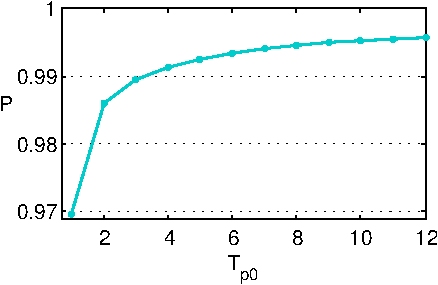
\includegraphics[width=3in]{Pictures/Compression/f1-crop.pdf}\\
  \caption{频域前12个系数的能量分布。}\label{Fig:Characteristic1}
\end{figure}


\item{高频信号中存在显著峰值:}\\
和其它自然信号(如图像)一样,胞外信号的主要能力也集中在低频部分。然而,这样的信号在中高频有所差异。如图\ref{Fig:Characteristic2}所示为中频部分的一部分截断光谱,可见在7325Hz处有一个明显的峰值,对应于一个经常出现的神经元放电模式。实际上,实验表明很多通道共享这些具有峰值的频率,而一些通道没有。这可以从多电极阵列的采样原理理解,我们采集到的胞外信号的单通道信息可以由3至5个有不同spike激发模式的神经元组成。

\begin{figure}[htb]
  \centering
  % Requires \usepackage{graphicx}
  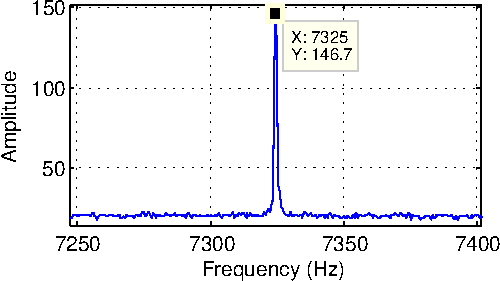
\includegraphics[width=3in]{Pictures/Compression/f2-crop.pdf}\\
  \caption{神经电信号高频部分DCT系数幅值分布。}\label{Fig:Characteristic2}
\end{figure}


\item{不稳定的通道间信号相关性:}\\
在\cite{Chen}的工作中Chen等利用了老鼠S1区采集信号的通道间相关性达到了较高的压缩效果。受此激发,我们也来研究一下在哺乳动物的运动皮层是否存在这样的相关性。

将原信号分为10个等长连续段,用$\bm{F}=\bm{\{F^1, F^2,\ldots, F^{10}\}}$表示这10段在频域的平均DCT系数,$\bm{F^{i}}\in R^{N_c\times S_b}$表示第i段的平均DCT系数大小,$N_c$为channel数目,$S_b$表示待转换为频域的信号长度。对于每个$\bm{F^{i}}$,我们计算其两两通道间的相关系数,记$\bm{C} \in R^{N_c\times N_c}$。图\ref{fig:Characteristic3}(a)(b)显示了一个时间序列段内频域的96个通道的两两相关系数矩阵,矩阵中,(i,j)位置的值表示 $i_{th}$ 通道和 $j_{th}$ 通道之间的相关系数,越深表示相关性越大,可见相关性变化很大。用变换系数(coefficient of variation)衡量相关系数的相对离散程度:


\begin{equation}\label{Eq:CV Definition}
  CV=\frac{\sigma}{\mu}
\end{equation}


其中 $\sigma$和 $\mu$分别表示相关系数的标准差和均值。当一个信号的$\sigma$相对$\mu$可忽略不计时,即CV很小时,称信号为稳定信号。对每个时间段$\bm{F^{i}}$,$\bm{CV}\in R^{N_c\times N_c}$衡量相关矩阵\textbf{\emph{C}}的浮动区间。$CV$的均值显示在图\ref{fig:Characteristic3}(c)中, 它是数据集中所有时间序列段内$CV$矩阵的平均值。 (i,j)位置的高度表示$CV$矩阵中$i_{th}$ 通道和 $j_{th}$ 通道相关系数的平均值。 这$N_c\times N_c$个$CV$的均值为0.68, 也就是说, 相关系数随时间剧烈变化, 所以在我们获得的运动皮层神经信号中, 通道间的相关性并不稳定,所以也较难将其应用在减少通道间冗余上。


\begin{figure}
  \centering
  % Requires \usepackage{graphicx}
  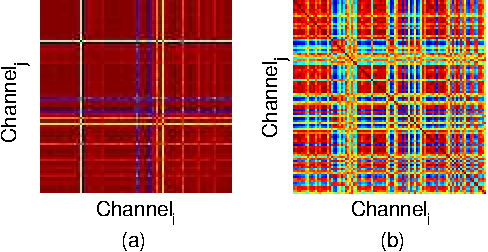
\includegraphics[width=3in]{Pictures/Compression/f3(ab)-crop.pdf}\\
  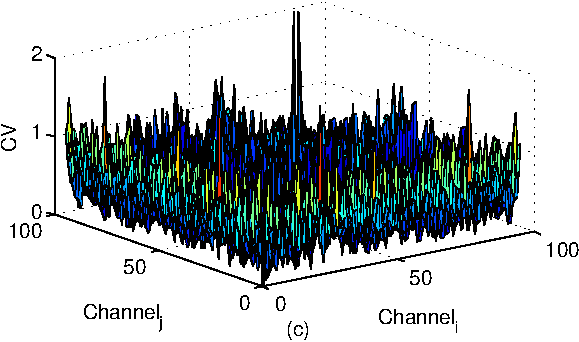
\includegraphics[width=3in]{Pictures/Compression/f3(c)-crop.pdf}\\
  \caption{通道间相关系数。 }\label{fig:Characteristic3}
\end{figure}

\end{enumerate}



\section{提出方法概括}
这篇文章中,我们考虑到上述信号特征,提出了一个高保真神经电信号压缩框架。首先,由于通道间相关性不稳定,我们对每个通道的信号做独立处理。整个框架的示意图见图\ref{Fig:Compression Algorithm Diagram}。它包括两个连续模块:"预处理"和“双阶编码”。

\begin{figure*}
  \centering
  % Requires \usepackage{graphicx}
  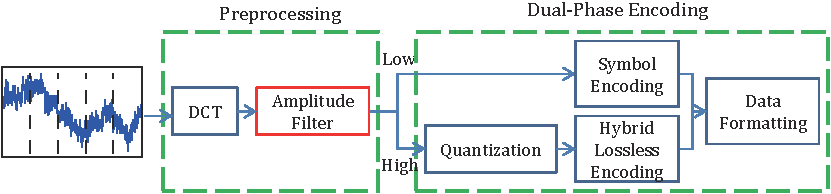
\includegraphics{Pictures/Compression/f4test1-crop.pdf}\\
  \caption{Flow diagram of the overall compression algorithm}\label{Fig:Compression Algorithm Diagram}
\end{figure*}

对于每个通道,首先将原信号分割成长度为$S_b$的块,然后每块通过以下两个模块进行处理:\\
\begin{enumerate}[\sffamily a.]
\item{\textbf{\textit{Preprocessing}}}\\
该模块通过离散余弦变换(Discrete Cosine Transformation,DCT)将原信号转换成频域。由于高频部分一些峰值可能对应于spike firing模式,所以传统压缩方法不适用于该信号的压缩。因此,我们提出按频谱幅值对信号进行分割,而不是根据频率高低分割。DCT系数通过一个幅值滤波器,分为高幅值成分(High-Amplitude-Component,HAC)和低幅值成分(Low-Amplitude-Component,LAC)。HAC包含显著地LFP和动作电位,其他信号归入LAC。 
 
\item{\textbf{\textit{双阶编码}}}\\
在神经信号的研究分析中已有证明,一个神经元完全由其神经元受刺激后的信号发放频率firing rate刻画\cite{32}。信号发放频率为单位时间内的动作电位发放个数。这个概念在2007年被\cite{3}中做出了修正,其中声明将LFP和spike结合起来可以加强神经信号解码准确率。也就是说,高幅值成分对神经信号表达更重要,因为这部分包含LFP和spike活动。相反,低幅值部分有效性较弱,但我们为了全局信号保真度和后续研究,也应在压缩时予以保存。这里我们提出双阶编码模块,它可以同时保存HAC和LAC的信息。在第一个阶段,低幅值部分由符号编码进行压缩,每个LAC中的DCT系数由1bit的符号表示;第二个阶段中,先将高幅值部分量化到一个相对小的范围区间,在通过我们提出的无损混合编码策略进行压缩。
\end{enumerate}









\section{双阶编码}
双阶编码模块的提出就是为了在压缩过程中同时保存全局和局部神经电信号。它对预处理信号定义了两个独立的操作。第一个阶段采用有损压缩策略,通过符号编码压缩低幅值部分,在这个阶段,16bit的原始信号值通过平均值平滑由1bit的符号表示。在第二个阶段,将DCT系数中LAC部分置零。所得到的向量中包含HAC部分量化后通过一个混合编码方法进行压缩。该编码方法将哈夫曼编码和我们提出的零长编码进行混合。哈夫曼编码处理高幅值项,而零长编码处理向量中的零元素。通过混合编码对LAC和HAC分开压缩可以有效地保存LAC和HAC的频谱位置,而无需存储多余信息。最后,对这两部分生成的编码进行格式化存储。
 
 
 
\subsection{符号编码}
\label{sec:Symbol Encoding for Low-Amplitude Component}
在双阶编码模块的输入端,信号通过一个幅值滤波器。为了达到高压缩率,低幅值部分通常直接被舍弃。但这样的话大块丢弃的系数容易引发很大重构误差,从而影响信号保真度和后续研究。为了解决这个问题,我们为该部分提出了一个有效的表示方法。

在神经信号解码的研究中,从带噪声的数据中预测神经元响应是一大难题:给定相同的刺激,但神经元几乎没有两次会出现相同的活动模式。为了准确表示神经元表达,需要对信号做一些均值平滑处理 \cite{31}。因此,均值通常用来代表原始系数,受这个激发,我们这里也在压缩过程中用信号的均值代替。

在符号编码中,均值在频域进行操作。低幅值DCT系数用其均值表示。由于正负系数进行平均可能被抵消,因此我们存储的是幅值,即系数的绝对值。为了有效压缩,各通道LAC部分的平均幅值预先计算好,然后用1-bit的符号表示其正负。记LAC中元素i为$l_i$,其符号表示为:

\begin{equation}\label{Eq:symbol definition}
  symbol(l_i)=\left\{
    \begin{array}{lr}
        -1,\ -T_{LH}<l_i\leq 0\\
        1,\ 0<l_i<T_{LH}
    \end{array}
  \right.
\end{equation}

其中-1,1位系数符号,-1示负,1表示正,$T_{LH}$表示低幅值和高幅值之间的分界阈值。根据公式\ref{Eq:symbol definition},含有$S_l$个元素的LAC向量通过符号编码被压缩为$S_l$个bit的向量,用来在解码时恢复。

在压缩解码时,我们将每个元素的编码符号乘以其幅值即可。这里有一个问题就是如何恢复LAC部分元素的位置。我们可以直接存储其位置,但是这样太耗费空间。事实上,我们无须显式存储其位置。由于LAC部分已经被编码,我们可以在待压缩信号中将其置零,而后续处理中只要保证其他压缩元素都非零即可,这样,在解码时只要找出所有零项即可恢复LAC。



\subsection{量化}
由于HAC部分包含LFP和主要spike,这个重要部分要比LAC做更精细的保存。为此,这一块信息线被量化到一个小区域,然后通过一个混合编码方法进行压缩。本节中介绍第一步操作——量化。当信号从预处理模块输出是,每个长为$S_b$的数据块通过一张量化表进行量化。这本身是一个有损压缩过程,但是通过共享量化表可以丢掉部分冗余信息。量化定义为原始信号除以对应的量化值,然后取整。这些量化值在不同信号通道又不同取值,从而组成量化表(Quantization Table, QT)。令$QT\in R^{N_c\times S_b}$表示量化表,其中$N_c$表示通道数,$S_b$表示数据块大小。记量化后第c项为$H_c^Q$,有

\begin{equation}\label{Eq:Quantization Step}
  H_c^Q=round(H_c./QT(c,:)),
\end{equation}

其中./是一个向量逐项除法,$round(x)$为取整操作,返回距离x最近的整数。注意,$H_c$中的元素幅值都大于等于$T_{LH}$,所以只要能令$ QT(c,:)$中的元素都小于$T_{LH}$,那么量化后,HAC的绝对值就都大于等于1了,这样可以很好地分离压缩后信号中的LAC分量和HAC分量。

对于待量化的高幅值部分,其取值范围由信号和$T_{LH}$共同决定。然而,神经电信号会因个体差异而拥有不同的采集信号取值\cite{33}。而且,不同神经元拥有不同的频谱分布,因此需要对每个个体的不同通道建立特定量化表。在符号编码中我们已经计算了LAC的平均幅值,这里我们将其用于量化表。

该量化表的设计出于以下几点考虑。一,考略到个体差异性,我们给每个实验个体建立独一无二的量化表。二,我们在研究运动皮层神经电信号特性时讲到过不同通道具有不同皮普分布,因此量化分量在通道间不共享。三,由于取整操作,转换后的取值有所变化,但是变化幅度不会大于对应位置量化值的$\frac{1}{2}$,不会损失太多信息。而且,这样量化表的值也可以都小于$T_{LH}$,使得量化后结果不小于1,满足了\ref{Symbol Encoding for Low-Amplitude Component}节中提到的非零特性。



\section{混合无损编码}
由于高幅值部分所有元素在量化后都成为了整数,离散分布的信号可以通过编码无损压缩,该无损压缩可由哈夫曼编码和零长编码方法实现。

作为最优符号编码方法,哈夫曼编码生成最佳可变长码,可以有效运用在我们量化后的数据上。然而,很多高频部分DCT系数的幅值都很小,容易被归入LAC分量。经过幅值过滤器处理后,很多高频参数在HAC中变成了0.因此,可以通过将高频部分连续的0替换成0的个数达到更好的编码效果,这就是零长编码的思想。于是,所有非零DCT系数都可以与哈夫曼编码表示;设置一个界限$B$,$B$之前的零用哈夫曼编码方法,$B$之后的零用零长编码分别进行表示。为了有效结合这两种方法,$B$的设定就很重要了,而它的取值取决于零的分布。为了更清晰地描述我们提出的混合编码方法,我们首先介绍一下哈夫曼编码和零长编码,然后来看怎样设置临界点$B$。


\subsection{Huffman编码}
熵编码方法是一种无损压缩技术,通常为每个符号创建一个独一无二的码。作为最常用的熵编码方法,哈夫曼编码\cite{22}用在我们的无损编码部分,旨在建立一棵最优树,能够最小化加权树高和(即信号编码总长度)\cite{21}。为了将原始值转换成二进制序列,哈夫曼编码方法基于每个符号的出现次数进行编码。

首先来看计算DCT系数的分布。根据我们的实验,HAC系数服从高斯分布,而很高的幅值非常少,那么为所有系数建立哈夫曼编码就是一件既耗时又浪费空间的做法,因为首先要计算其哈夫曼编码,而后由于其频率太少,会导致码字很长,浪费空间。因此我们并非计算所有DCT系数分布,对于非零系数,我们只计算$[-Z,Z]$的部分,其中$Z$是系数的统计范围。而超出该范围的幅值,我们单独记录其值和位置。此外,并非所有系数零都予以统计。令\emph{B}表示哈夫曼编码与零长编码之间的分界点,由于只有\emph{B}之前的零采用哈夫曼编码,我们就只统计\emph{B}之前出现的零的个数。




\begin{figure}
  \centering
  % Requires \usepackage{graphicx}
  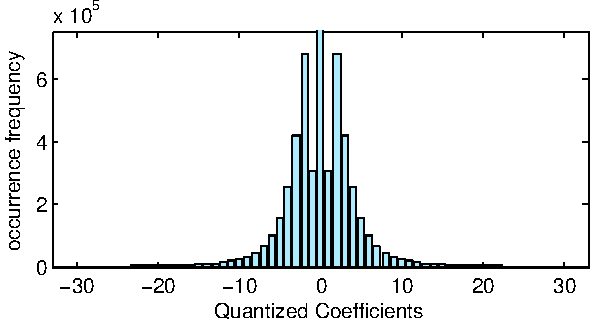
\includegraphics{Pictures/Compression/f5-crop.pdf}\\
  \caption{频域量化系数。}\label{fig:Quantized Coefficient Distribution}
\end{figure}


统计幅值在$[-Z,Z]$内所有非零系数以及$B$Hz前零元素的分布,将$N_c$个通道求得平均,如图\ref{fig:Quantized Coefficient Distribution}所示, 其中横轴表示[-31,31]的整数系数范围,纵轴表示量化后每个系数的出现次数。在这个例子中,$B$由\ref{Delimitation of Quantized Data}节中的定界策略决定。根据这个统计结果,哈夫曼编码对这些系数进行编码。



\subsubsection{零长编码(Zero-Length-Encoding)}
\label{Zero-Length-Encoding}

零长编码方法为了对高频部分连续的零进行编码。我们用八进制表示法表示连续$k_z$个零,用哈夫曼编码来分隔两个相邻的八进制数字。举例,$k_z=(8A+B)\times 8+C$,其中$A$, $B$, $C$ 分别表示三阶,二阶,一阶的八进制数字。用\textbf{\emph{HCT}}表示哈夫曼码表(Huffman Code Table), 即DCT系数的不定长编码表,混合编码格式如下:

\begin{figure}[H]
  \centering
  \caption{混合编码格式示例}
  % Requires \usepackage{graphicx}
  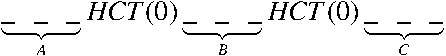
\includegraphics{Pictures/Compression/HCT-crop.pdf}\\
\end{figure}

令$g(k)$为要表示的0个数所需阶数,我们有


\begin{equation*}
  g(k_z)=\left\{
    \begin{array}{lr}
        1,\ k_z\in[0,7]\\
        2,\ k_z\in[8,7\times8+7]\\
        3,\ k_z\in[64,63\times8+7]\\
        \ldots
    \end{array}
  \right.
\end{equation*}


可以规范化为:
\begin{equation}\label{Eq:g(kz) definition}
  g(k_z)=\left\{
    \begin{array}{lr}
        1,k_z=0\\
        \lceil \log_8(k_z+1) \rceil,else
    \end{array}
  \right.
\end{equation}

在解码过程中,首先读入一个3-bit二进制码字,然后检测下一个序列是否和$HCT(0)$相同。如果是,就再读三位,以此类推,直到条件不满足为止,这时就可以计算该段有多少个连续0了。由于哈夫曼编码是前缀无歧义编码(prefix-free code), 所以可以保证零的表示不会出现歧义。

零长编码通过直接编码连续零,而非一个个表示来节省空间,因此我们希望零长编码的信号段拥有更多连续的零(而不是分散的),因此确定一个好的分界点$B$尤为重要。








\subsection{混合无损编码分界}
随着量化信号中连续零数量的增多,可以想见零长编码要比哈夫曼编码短,为了证实这个想法,我们来看混合编码策略中两种编码方法的编码。

对分界面的简单估计可以通过计算零的个数分布而得。将每$S_b$个离散时间序列点分为$N_s$个等长短序列段,然后计算每段中零的个数。图\ref{fig:Zero Distribution}显示了1600个DCT系数分割为16段($S_b$=1600, Ns=16)的零数分布, 对于 $S_b=1600$, 将1600个元素分为16段,每段有100个分量。黄色和蓝色线条分别表示每段中零元素个数的均值和方差。 可以看出零的个数分布随着频率而增多。用$\Omega_0\in R^{N_s}$表示平均零数分布,即图中的黄色条,则可以根据零数分布情况进行分界。

\begin{figure}
  \centering
  % Requires \usepackage{graphicx}
  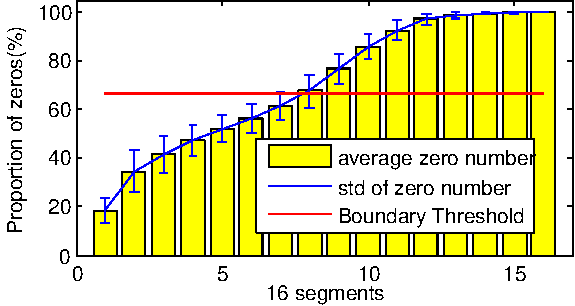
\includegraphics{Pictures/Compression/f6-crop.pdf}\\
  \caption{16个序列段的零元素分布情况。}\label{fig:Zero Distribution}
\end{figure}

令$T_{HZ}$表示在哈夫曼编码与零长编码的分界$B$处,零的出现概率,那么该段中领的个数可以用$T_{HZ}\cdot \frac{S_b}{N_s}$表示,其中$\frac{S_b}{N_s}$是每段中的元素个数。这样,分界限可由式\ref{Eq:Boundary Brief Def}得出,$B$之前采用哈夫曼编码,$B$之后采用零长编码。

\begin{equation}\label{Eq:Boundary Brief Def}
  B=CrossSegment\left(\Omega_0,T_{HZ}\cdot\frac{S_b}{N_s}\right)\cdot\frac{S_b}{N_s}
\end{equation}

该式中,CrossSegment函数返回零的出现频率和阈值$T_{HZ}$的交点出数据段编号。图\ref{fig:Zero Distribution}中红色线表示阈值$T_{HZ}*(S_b/N_s)$,用来分隔混合编码中的两个算法, 图中可见零分布线(黄色)与阈值线(红色)交于第7段。该例中,$S_b$=1600, $N_s$=16, 定义 $T_{HZ}$=0.75,那么有$B$=700。


下面我们来仔细分析交点位置。用x表示交点段的编号,在式\ref{Eq:Boundary Brief Def}中直接用$T_{HZ}$乘以每段中的元素个数,而在式\ref{Eq:Boundary Precise Def}中,考虑到了交点段中阈值与段交点处所占的比例。


\begin{equation}\label{Eq:Boundary Precise Def}
  \begin{array}{lr}
    x=CrossSegment\left(\Omega_0,T_{HZ}\cdot\frac{S_b}{N_s}\right)\\
    B=\left((x-1)+\frac{T_{HZ}\cdot \frac{S_b}{N_s}-\Omega_0(x-1)}{\Omega_0(x)-\Omega_0(x-1)}\right)\cdot \frac{S_b}{N_s}
  \end{array}
\end{equation}


最后一个问题是$T_{HZ}$的设定。由于$T_{HZ}$表示在$B$处,系数零所占比例,它可以表示每个非零元素之前平均零的个数,即


\begin{equation}\label{Eq:T_HZ def}
  T_{HZ}=\frac{k_z(B)}{k_z(B)+1}
\end{equation}


其中的1表示非零系数,$k_z(B)$表示在分界线$B$处一个非零系数之前的平均零的个数。

基于DCT系数的统计特性,分界可以进一步提升压缩性能。然而,从上面的推导可知,在式Eq.\ref{Eq:Boundary Precise Def}和 \ref{Eq:T_HZ def}中,计算$B$和$T_{HZ}$是一个死锁。公式\ref{Eq:Boundary Precise Def}需要$T_{HZ}$的值,而$T_{HZ}$的值要在式\ref{Eq:T_HZ def}中由\emph{B}决定。为此我们提出了一个迭代检验方法,该法需要根据混合编码两种方法生成的码字长度合理确定界限的位置。

令$HCT$表示前面生成的哈夫曼编码表,
\textbf{\emph{HCT}}(x)表示x的哈夫曼编码,
$l_0\in Z_+$ 表示$HCT$码表中0的码字长度,
$k_z$ 表示一个非零元素之前0的平均个数。若量化系数全部由哈夫曼编码表示,其长度为:


\begin{equation}\label{Eq:length of Huffman}
  l_1=\sum_{i=1}^I [HCT(x_i)]+l_0\cdot k_zI,\ x_i\in H_c^Q, x_i\neq 0
\end{equation}


其中$I$是$H_c^Q$中所有非零系数集合的大小。该式中,第一项将所有非零元素$x_i$的长度进行加和,
而$l_0\cdot k_zI$ 表示所有‘0’的长度和,因为每个非零系数之前平均有 $l_0\cdot k_z$ 位数字。


类似地,如果量化系数中的零全部由零长编码表示的话,编码长度为:


\begin{equation}\label{Eq:length of Zero-length-Encoding}
  l_2=\sum_{i=1}^I [HCT(x_i)+(3+l_0)g(k_z)-l_0],\ x_i\in H_c^Q, x_i\neq 0
\end{equation}


根据零长编码格式\ref{Zero-Length-Encoding},$(3+l_0)$是八进制表示中每多一阶多需要的表示位数。用 $g(k_z)$ 表示$k_z$个零所需阶数,则 $(3+l_0)g(k_z)-l_0$ 可以表示一个非零元之前的零分量用零长编码所需长度。此处$k_z$并非确切平均零的个数,而是为了计算方便估计的最近整数。

To compare the two encoding length, we use Eq.(\ref{Eq:length of Huffman}) minus Eq.({\ref{Eq:length of Zero-length-Encoding}}) and take the part in the bracket as $f(k_z)$,

为了比较两种编码方法的长度,我们用公式\ref{Eq:length of Huffman}减去式\ref{Eq:length of Zero-length-Encoding},计入下式方括号内,即$f(k_z)$:


\begin{equation}\label{Eq:length difference}
  l_1-l_2 = \left[l_0\cdot k_z-(3+l_0)g(k_z)+l_0\right]I=f(k_z)\cdot I
\end{equation}


由于I是常数,我们只考虑以$k_z$为参数的函数f。将式(\ref{Eq:g(kz) definition}) 代入式(\ref{Eq:length difference}), 我们有


\begin{equation}\label{Eq:f(kz) Def}
  f(k_z)=\left\{
    \begin{array}{lr}
        -3,\ k_z=0\\
        l_0\cdot k_z-(3+l_0)\lceil\log_8(k_z+1)\rceil+l_0,\ else
    \end{array}
  \right.
\end{equation}


对于离散整数 $k_z$, 相邻项之间的差为:


\begin{equation}\label{Eq:f(kz)difference}
\begin{array}{lr}
  f(k_z)-f(k_z-1)=\left\{
    \begin{array}{lr}
        f(0)=-3;\\
        f(k_z)=f(0)+l_0k_z-(3+l_0)\lfloor\log_8{k_z}\rfloor
    \end{array}
  \right.\\
  \\
  where \ k_z\in Z_+,l_0\in Z_+
\end{array}
\end{equation}


由式(\ref{Eq:f(kz)difference})可得,$f(k_z)$只有在$k_z$最开始,即$l_0$不大于1时才会小于零。由于随着频率增加,$f(k_z)$有增加的趋势,所以$f(k_z)$与0只有一个交点,就是在 $\lfloor\log_8{k_z}\rfloor$ 等于零的时候。
在这个交点处,我们可得从式(\ref{Eq:f(kz)difference})得:


\begin{equation}\label{Eq:kz}
  k_z=\frac{3}{l_0}
\end{equation}


所以,混合编码中的阈值可以由式(\ref{Eq:T_HZ def})和 (\ref{Eq:kz})确定。 但是在参数选择过程中还有其他问题。正如我们之前提到的,在确定界限$B$,阈值$T_{HZ}$和哈夫曼编码表之中有死锁。
问题在于, $T_{HZ}$ 由 $k_z$ (式(\ref{Eq:T_HZ def}))计算而得,而$k_z$依赖 $l_0$ (式(\ref{Eq:kz})), $l_0$又由哈夫曼码表确定. 然而, \textbf{\emph{HCT}}需要计算 \emph B之前零的个数, 而这又由 $T_{HZ}$得来。为了打破这个死锁,我们再假设$l_0=1$下初始化$k_z$,见Boundary Descent 算法.

\renewcommand{\algorithmicrequire}{ \textbf{Input:}}      %Use Input in the format of Algorithm
\renewcommand{\algorithmicensure}{ \textbf{Output:}}     %UseOutput in the format of Algorithm
\begin{algorithm}
\caption{BOUNDARY DESCENT ALGORITHM}
\label{algo:bda}
\begin{algorithmic}[1]  
\Require Quantized HAC to be compressed $H_c^Q$
\Ensure  \textbf{\emph{HCT}},\emph{B}
\State	$k_z\leftarrow3,\varepsilon\leftarrow1$
\While{($\varepsilon=1$)}
    \For{$c\leftarrow1 to N_c$}
        \For{$i\leftarrow1 to S_b$}
            \State $\Omega_0(i)\leftarrow \sum_{c=1}^C 1_{\left\{H_c^Q[i]=0\right\}}$
        \EndFor
    \EndFor
    \State $T_{HZ}\leftarrow \frac{k_z}{k_z+1}$
    \State $x=CrossSegment\left(\Omega_0,T_{HZ}\cdot\frac{S_b}{N_s}\right)$
    \State $B=\left((x-1)+\frac{T_{HZ}\cdot \frac{S_b}{N_s}-\Omega_0(x-1)}{\Omega_0(x)-\Omega_0(x-1)}\right)\cdot \frac{S_b}{N_s}$
    \State $HCT\leftarrow Huffman Encoding(H_c^Q,B)$
    \If{($l_0(HCT)=\frac{3}{k_z}$)}
        \State $\varepsilon\leftarrow 0$
    \Else
    	\If{($l_0(HCT)\leq 3$)}
    	    \State $k_z\leftarrow \frac{3}{l_0(HCT)}$
    	\Else
	        \State $B\leftarrow 0,\ \varepsilon\leftarrow0$
	    \EndIf
    \EndIf
\EndWhile
\end{algorithmic} 
\end{algorithm}


算法\ref{algo:bda} 描述了界限下降算法的流程。令$\varepsilon$表示是否迭代的标志, $l_0(HCT)$ 表示哈夫曼码表中零编码长度,从假设 $l_0$(\textbf{\emph{HCT}})为1开始, 算法初始化$k_z$ 为3 (第一行)。只要迭代标志为真,就计算所有样本中的零分布(3-7行)。然后通过式(\ref{Eq:Boundary Precise Def}计算该方法的阈值 $T_{HZ}$ (第8行),然后根据式\ref{Eq:T_HZ def})计算混合编码中两种方法的分界点$B$ (9-10行)。以$\emph{B}$和量化信号$H_c^Q$作为输入,可获哈夫曼码表 \textbf{\emph{HCT}}(line 11)。
然后,检验最初的假设,即是否满足式(\ref{Eq:kz}). 如果迭代所得 $l_0$与假设不吻合,就用$\frac{3}{l_0}$代替,始终迭代直到达到条件$l_0$(\textbf{\emph{HCT}})$\cdot k_z = 3$ (12-16行)。注意$l_0$应被限制在3之内,否则就无须用哈夫曼编码了(17-19行)。这个算法最终返回 \textbf{\emph{HCT}} 和分界处 \emph{B}。

\begin{algorithm}
\caption{Overall Compression Algorithm}
\label{algo:overall_algorithm}
\begin{algorithmic}[1]  
\Require {$\bm{X}$, the signal; $S_b$, the block size; $T_{LH}$, the threshold between HAC and LAC; \emph{B}, the boundary within Hybrid Encoding}
\Ensure {$\bm{Y}$, formatted compression result; $\bm{Z}$, lengths of \emph{Symbol Encoding} codes for all blocks }
\State Divide $\bm{X}$ into blocks of size $S_b$, $\bm{X}_{(1)},\bm{X}_{(2)},...,\bm{X}_{(N)}$
%Calculate Quantization Table and LAC\\
    \For{$i = 1,...,N$}
        \State $\bm{F}_{(i)} \leftarrow DCT(\bm{X}_{(i)})$
        \State $\bm{low}_{(i)}\leftarrow$ find indices $(\bm{F}_{(i)}<T_{LH})$
        \State$\bm{LAC}_{(i)} \leftarrow F(\bm{low}_{(i)});\%\emph{LAC}$
    \EndFor
    \State $\bm{QT}\leftarrow$ average over $|\bm{LAC}_{(i)}|$,\,\,$i=1,...,N$
	\State $\bm{Y}$ $\leftarrow$ [\,]
\For{$i = 1,...,N$}
    \State $\bm{HAC}_{(i)} \leftarrow \bm{F}_{(i)}$; \,\,$\bm{HAC}_{(i)}(\bm{low}_{(i)}) \leftarrow 0$
    \State $\bm{S}\leftarrow sgn(\bm{LAC}_{(i)})$;\,\, $\bm{Y}\leftarrow [\bm{Y}\; \bm{S}];$  \%\emph{Symbol Encoding}
    \State $\bm{Z}_{(i)}\leftarrow length(\bm{S})$; 
    \State $\bm{H_c}^Q\leftarrow round(\bm{Hc}_{(i)}./\bm{QT});$
    \State $\bm{H}\leftarrow Huffman(\bm{H_c}^Q(1:B))$; $\bm{Y} \leftarrow [\bm{Y}\; \bm{H}];$
        \ForAll{$x \in \bm{H_c}^Q((B+1):end)$}
        	\If {$x\neq 0$}
            	\State $\bm{Y} \leftarrow [\bm{Y}\; Huffman(x)]$
	        \Else
    	        \State $\bm{Y} \leftarrow [\bm{Y}\; ZeroLength(x)]$
    	    \EndIf    	        
        \EndFor
\EndFor
\end{algorithmic}
\end{algorithm}


通过算法\ref{algo:bda} 求得压缩框架的全部参数后,我们用算法\ref{algo:overall_algorithm}总结一下整个算法的流程。 首先将信号以$S_b$为大小分割成$N$块,对于每个数据块,分别映射到频域,求DCT系数,求取$LAC$分量并按符号编码方法压缩(2-6行)。根据LAC分量幅值确定每个通道的量化表$QT$(第7行)。 然后对于每个块,对$LAC$分量编码,生成$HAC$分量并量化压缩,对混合编码分界点$B$之前的分量进行哈夫曼编码,对$B$之后的零分量进行零长编码,非零分量进行哈夫曼编码(10-21行)。最后返回编码$\bm{Y}$。







\subsection{编码格式化}
本节中,我们讨论数据的格式化存储。在前面的与处理步骤中已经提到,每个通道的信号首先在时域上分成很多数据块,每个数据块包括$N_c$个通道,如图\ref{fig:Data Format}所示。

根据三个二进制编码方法,每个通道的码字包括哈夫曼编码,零长编码和符号编码三部分结果。对于高幅值分量,假设哈夫曼码表中有$HCT(0)=1, HCT(3)=010, HCT(-6)=110010$, 对哈夫曼编码部分,借助$HCT$进行解码,对零长编码部分,由于$k_z$个0用$(3+l_0)g(k_z)- l_0$ 位来记录,所以也可以根据表示位数进行解码。 举个例子,加入我们现在拿到的编码结果为:"0101110", 那么在哈夫曼编码中,该码字表示的就是3,0,-6;而零长编码中,该码字则表示22(22=2*8+6)个零,后面跟一个3。当我们将HAC部分解码完毕后,LAC在最后进行解码,表示每个值的正负,如图\ref{fig:Data Format}所示。

在编码过程中,由这三种编码而得的是一个二进制流。但是我们需要将这三种编码的结果分离开才能进行解码,因此在码字最开始的地方我们记录两个位置,一个是哈夫曼编码和零长编码的边缘,一个是零长编码之后,符号编码之前的分离点。此外,我们还需要记录的是每个个体的对应的量化表。


\begin{figure}
  \centering
  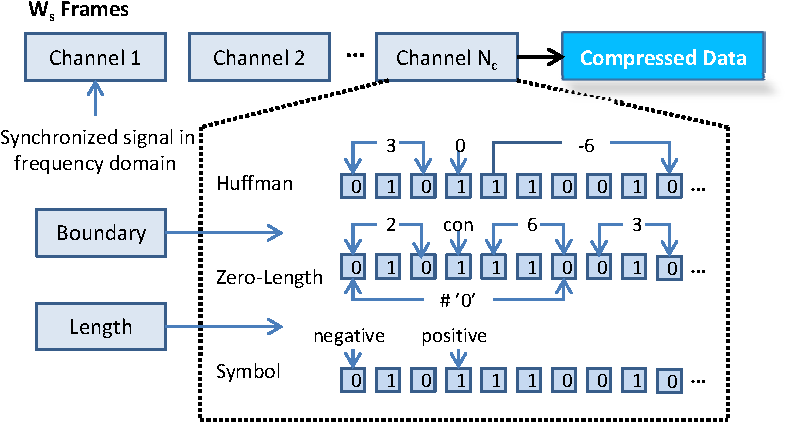
\includegraphics{Pictures/Compression/f8-crop.pdf}\\
  \caption{压缩数据格式化}\label{fig:Data Format}
\end{figure}





\section{实验}
这一节展现我们的实验结果,数据基于过去四年从两只猴子采集的数据。我们讨论了参数设定问题,并与经典信号压缩算法做了比较。

\subsection{数据集}

我们的实验数据及采集自浙江大学求是学院BMI系统 \cite{14}。为了训练猴子,建立了一套训练系统,该系统中,每只猴子在一个从中心出发的四方向摇杆上做训练,目标是根据可视的提示将方向杆摇至正确方向。完成了这项任务后,会对猴子大脑运动皮层(M1区)植入一个多电极阵列来捕捉手摇杆动作所产生的神经信号。每次试验持续大概60分钟。

这项任务在一个多通道捕获设备(Cerebus 128TM (Blackrock Microsystem, Salt Lake City, UT, USA))上完成,同时记录106个神经元的信号。 信号在96个电极(电极长1.0mm,总长度7.0cm)上进行采样,即以30kHz为采样频率,采96个通道,16-bit的分辨率。这样实验所获数据流为5.76MB/s, 也就每5分钟获得1.73GB的数据。为了检验我们的压缩算法,我们随机选择了12条记录,没条记录长300秒。




\subsection{评价标准}
为保证神经电信号压缩后的可用性,压缩算法在减少信息所占空间的同时希望保证重构信号的相对信息完整\cite{24}。从这个角度出发,我们需要一些压缩的评价标准来度量压缩效果。

\begin{enumerate}
\item{Signal to Noise Ratio}\\
在信息论中,信噪比(Signal to Noise Ratio, SNR)用来评判信号压缩的保真度。

令 $S_o$ 和 $S_r$ 分别表示原始信号和重建新号, SNR定义为$S_o$与$S_o-S_r$的能量比:


\begin{equation}\label{Eq:SNR Def}
  SNR(S_o,S_r)=10\cdot \log_{10} \frac{\left\|S_o\right\|_2^2}{\left\|S_o-S_r\right\|_2^2}
\end{equation}

作为一个基于能量的评判标准,SNR可以很好地反应误差的能量,但这还是不够的。回想我们在第\ref{Characteristics}节中分析的第一条信号特性,信号的主要能量集中在低频区域。也就是说低频区域对SNR影响很大,而这对高频区域就不平等了。为了解决这个不平等问题,我们将在另外的评判标准中聚焦于spike信号,也就是高频部分的主要有效信号。

\item{Spike ratio}\\
为了检验spike的保留程度,我们引入Spike Ratio, 表示一段信号与其压缩后重建新号相比保留的spike比例。在我们的验证中,常用的幅值阈值技术\cite{34}用来检测spike,其中阈值$Thr$设定为:


\begin{equation}\label{Eq: Spike Detection Threshold}
  Thr=\alpha \cdot \sigma_n,\ \sigma_n=median\left(\frac{|x|}{0.6745}\right)
\end{equation}

其中 $\alpha$ 是一个常量银子, $\sigma_n$ 是背景噪声的标准差估计量. 如果一个点的值大于 $Thr$,就视其为一个spike的起始点。 注意计算spike不留程度不是一个计数问题,而是计算匹配的spike个数,也就是有多少spike保留在了正确的位置。在此过程中,我们分别在原始信号和压缩重建新号上检测spike,并计算Spike Ratio。

为了帮助理解重建效果, 图\ref{fig:Criterion Comparison}给出了一小段截取的数据在不同SNR和Spike Ratio上的压缩结果,其中黑线表示原始信号, 蓝色和绿色线表示重构信号,检测到的显著spike标注为下方的短线段。 图中(a). 蓝色线的重构效果: SNR = 31.02, Spike Ratio = 80\% (b). 绿色线的重构效果: SNR = 36.68, Spike Ratio = 100\%。 底部竖线段表示检测出spike的对应位置。


 可以看出,在右图中x=779处检测到的spike并未在左图中检测出来。这是因为信号在这里压缩时有一部分被丢掉了, 以至于在spike检测的时候没有达到式\ref{Eq: Spike Detection Threshold}中的阈值。 注意高SNR经常伴随着高Spike Ratio, 但也不一定总成立。因为SNR更多的反映了信号在低频能量上的特点。 


\begin{figure}
  \centering
  % Requires \usepackage{graphicx}
  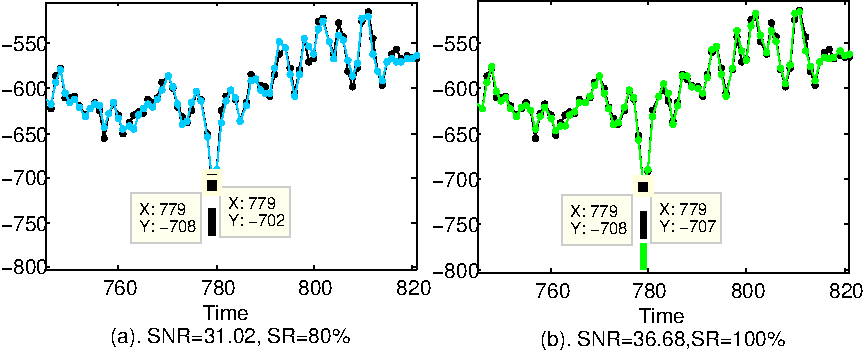
\includegraphics{Pictures/Compression/f9-crop.pdf}\\
  \caption{截断数据段的两个重构效果对比示意图。}
\end{figure}



\item  Compression ratio
此外,我们还用压缩(Compression Ratio, CR)比来从数据冗余减少情况的角度度量压缩效果。压缩比定义为信号的压缩后大小除以原始信号所占空间。

\end{enumerate}

在下面的实验中,我们在以上三个评价标准上来衡量压缩算法的有效性。





\subsection{参数设置}
本小节中,我们讨论如何选定三个参数:  $T_{LH}$, 幅值过滤器的阈值; $\omega$, 量化表的比例; 和 $S_b$, 预处理中每个数据块的大小。


在我们提出的压缩框架中,有两个步骤会造成信息丢失:一是符号编码中的均值代替策略,而是高幅值分量的量化。这两个步骤都是在频域操作的,但是符号编码环节中,信息丢失最大为相应的量化表的值;而量化部分信息丢失最大为量化表对应值的一半。具体用哪一种方法进行压缩取决于高低幅值分量之间的界限,也就是取决于幅值滤波器的阈值$T_{LH}$。随着$T_{LH}$的升高,会有更多分量被符号编码压缩,带来更大的信号损耗而提高压缩率。因此,$T_{LH}$可以看做是重构效果和压缩比之间的协调系数。在我们的模拟中,$T_{LH}$在整个数据集上测试,以求的最佳的压缩效果。

另一个重要参数是量化表。为了在压缩过程中节省参数,量化表以LAC分量的平均幅值作为结果,在符号编码中进行共享。因此,QT会随着$T_{LH}$的增加而增加,从而在量化过程中可以粗化数据,降低其分辨率。 这里我们想了解能否通过调整QT的比例达到更好的压缩效果。 所以, 我们用QT乘以一个比例系数$\omega$来调整QT进行试验,其中,$\omega$在 $[0.5,2.5]$之间,以0.5为步长进行测试。


在不同参数下,我们的实验结果如图\ref{fig:Comparison-TLH}所示。 每个字图的横轴都是阈值 $T_{LH}$ . 不同大小的量化表用比例系数$\omega$表示, 其中 $\omega$ = 0.5(—), 1 (---), 1.5 (…), 2(-.-.-) and 2.5(-*-*-)。 每个子图的结果都是通过系统地调节阈值$T_{LH}$和比例系数$\omega$,然后在整个数据集上做结果的平均而来的。保持$\omega$不变,随着$T_{LH}$的上升,可以清楚地看到SNR和Spike Ratio都有所下降,这是因为高阈值会同时放大QT,相反这样会带来更优的压缩率。从图中可以看出,从SNR和Spike Ratio的角度来看,$\omega=1$ 的结果总是最优的;从Compression Ratio的角度来看,$\omega=1$的配置排在第二。容易理解为什么Compression Ratio随着$\omega$的增大而变化(降低), 因为$\omega$更意味着损失更多数据,导致Compression Ratio降下来。


\begin{figure*}[htb]
  \centering
  % Requires \usepackage{graphicx}
  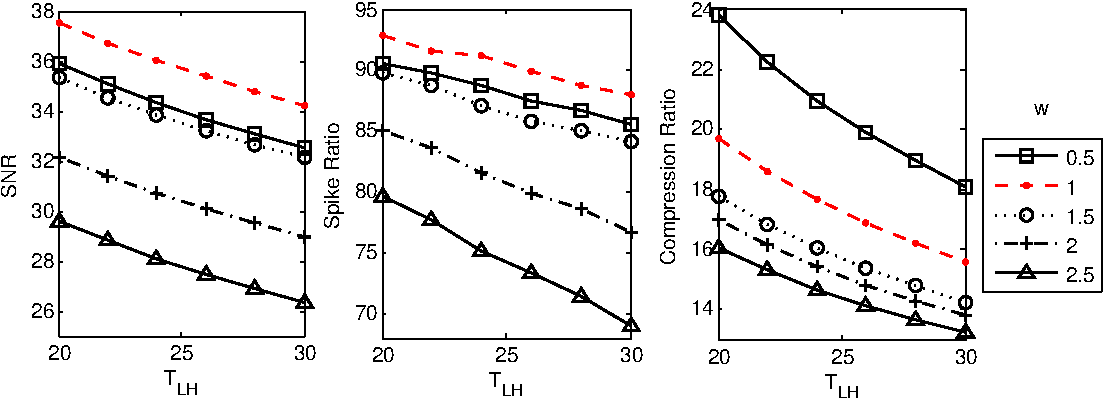
\includegraphics[scale=0.9]{Pictures/Compression/f10-crop.pdf}\\
  \caption{ 不同$T_{LH}$和QT下的 SNR, Spike Ratio 和 Compression Ratio。}\label{fig:Comparison-TLH}
\end{figure*}


图\ref{fig:Comparison-TLH} 展现了$\omega$是怎样影响压缩比和信号保真度的,但是由于没有一个$\omega$在3个评价指标上都达到最佳结果,所以我们仍然很难评判哪个$\omega$最好。 为此,图\ref{fig:Comparison:TLH-2}直观地表示出,在相同Compression Ratio的情况下,另外两个压缩评价标准的值。 该图是图\ref{fig:Comparison-TLH}的一个变换,图中横轴以压缩比作为自变量, 纵轴 (a). SNR, (b). Spike Ratio作为因变量, 每条曲线表示在不同QT的比例系数和阈值下的压缩效果。 可见,在相同Compression Ratio下$\omega=1$总是达到最好的效果。因此,对于无监督压缩,QT的比例系数为1时可以权衡压缩率和重构效果,给出一个理想的压缩结果。


\begin{figure*}[htb]
  \centering
  % Requires \usepackage{graphicx}
  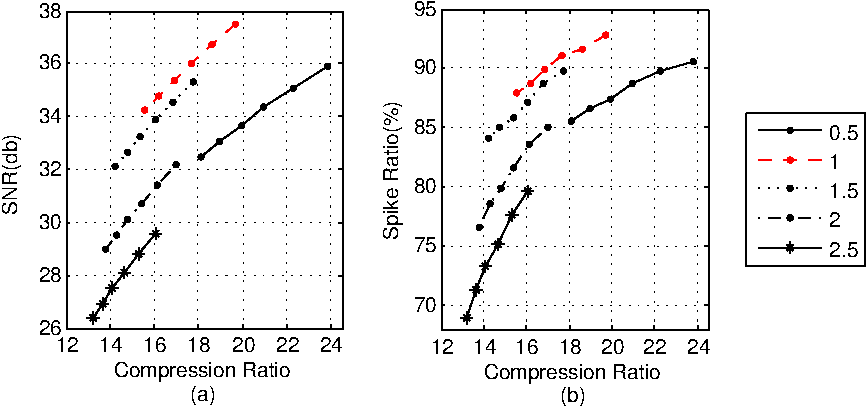
\includegraphics[scale=0.9]{Pictures/Compression/f11-crop.pdf}\\
  \caption{不同量化表比例系数下的压缩效果。 }\label{fig:Comparison:TLH-2}
\end{figure*}

$T_{LH}$的选择取决于我们的压缩要求。例如, 如果希望SNR大于30db且Spike Ratio不小于90\%的话,选择$T_{LH}=24$, 可以得到平均Compression Ratio为17.75\%, SNR达到36.24db, Spike Ratio大于90\%。 

最后需要确定的参数是预处理中的数据块大小$S_b$了。 在上述实验中,我们暂时都取$S_b = 1600$, 这里我们来讨论能否通过更改$S_b$达到更好的压缩效果。 实验结果如图\ref{fig:Comparison:Sb}所示, 其中横轴表示块大小$S_b$, 固定$T_{LH}=24$, $\omega$=1,  $S_b$ 在 1500 到 28500之间进行测试。


\begin{figure*}[htb]
  \centering
  % Requires \usepackage{graphicx}
  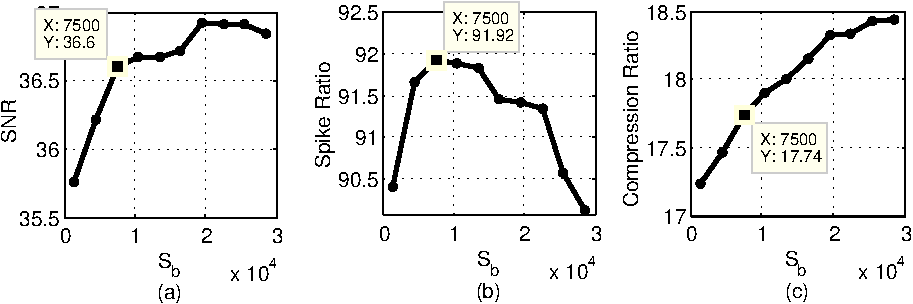
\includegraphics[scale = 1.1]{Pictures/Compression/f12-crop.pdf}\\
  \caption{不同块大小$S_b$下进行数据分割的压缩预处理的压缩结果。}\label{fig:Comparison:Sb}
\end{figure*}


该图说明随着$S_b$的增长,信号的保真度先提高后下降。原因如下:
首先,更大的$S_b$会使DCT系数更为精确,于是在IDCT(inverse DCT)的过程中降低误差。 但是, 这样会生成很多低幅值的DCT系数, 这样会使得归入LAC分量的值增多,也就是, 会有更多分量选用符号编码方法进行压缩, 这使得loss增大。 因此, 压缩保真度先增后减反映了上述两个因素之间的平衡。 根据给定的实验结果, 可以将数据块最佳大小设置为$S_b = 7500$, 这时达到整个数据集上平均Compression Ratio为17.7\%, SNR为36.6db, Spike Ratio为91.9\%。


\subsection{符号编码有效性}
在第\ref{sec:Symbol Encoding for Low-Amplitude Component}节中,我们提出了符号编码方法来压缩低幅值的DCT系数。 本节中给出实验结果, 探讨符号编码的有用性。 在上一节中我们已经选出最佳参数。 给定这些参数设置, 我们设计一个对比试验, 保持高幅值部分压缩方法不变, 对低幅值部分不采用符号编码而是整个丢弃, 以此来看符号编码所带来的改善。 比较结果如表格\ref{tab:T1}所示。\\


\begin{table}[ht]
\centering
  \begin{tabular}{c c c c}
  \hline\hline
  符号编码 & SNR(db) & SR & CR \\ [0.5ex] %insert table heading
  \hline
  有 & 31.4 & 83.7\% & 13.1\% \\
  无 & 36.6 & 91.9\% & 17.7\% \\
  \hline
  \end{tabular}
  \caption{SNR, Spike Ratio and Compression Ratio With and Without Symbol Encoding (Low-Amplitude)}
  \centering \label{tab:T1}
\end{table}


可以清楚地看出, 将低幅值分量考虑进来可以保存很多有效信息。 虽然这样会升高Compression Ratio, 但从SNR和Spike Ratio的角度来看,通过符号编码后重构效果有了很大提升。 这是由高频部分系数的内部分布决定的。 因此, 高频部分的符号编码是一个有效的压缩方法。



\subsection{方法比较}
由于在神经电信号压缩方面缺少统一的压缩标准作参照,而音频也是单维度时序信号, 所以我们在本节中选择与state-of-art的音频压缩算法作比较。 同时,我们也与其他传统数据压缩方法作比较。 通过与有损和无损压缩算法比较的试验结果可得,我们的压缩算法能够权衡重构效果和Compression Ratio。


\subsubsection{无损压缩}
本小节中讨论无损音频压缩和通用数据的压缩技术。无损压缩方法通过更为紧凑的编码格式对原文件进行编码, 使得数据编码后解压所得文件与原文件完全一样。 对音频压缩, FLAC之类的编码方法利用线性预测来估计信号频谱,可以对通用波形的Compression Ratio达到50\%到60\%\cite{23}。 但是神经信号不同于音频信号, 神经信号更为复杂,难以预测。 所以这类压缩方法即便用到神经信号压缩, 也不能获得较好的Compression Ratio。 类似的, 通用数据文件压缩方法, 如 Zip, 7-Zip 和 RAR 也不能达到相对较低的压缩率。 表\ref{} 显示出不同无损压缩技术的
压缩比。可见,在神经信号上最好的压缩方法是APE (Monkeys Audio), 得到最小压缩率为56.88\%。 注意,尽管神经信号被这些方法压缩后不能得到很好的压缩率, 但文件可以被完好的重建出来, 因此, SNR 是无穷大。 


\begin{table*}[ht]%开始表格
\caption{无损压缩方法性能比较} % 表格的名称
\label{tab:T2} \centering
\begin{tabular}{|c||c|c|c|c|c|c|}%开始绘制表格
\hline
 & \multicolumn{5}{c|}{无损压缩编码} & Ours\\
  \hline \hline
 \multirow{2}{*}{类型} & \multicolumn{3}{c|}{音频编码} & \multicolumn{2}{c|}{文档文件格式} & SNR=36db\\
 \cline{2-6}
 & Lossless WMA & FLAC & APE & Zip & RAR &Spike Ratio=92\%\\
 \cline{1-7}
 压缩比 & 70.89\% & 54.27\% & 53.08\% & 70.04\% & 60.91\% & 17.74\%\\
\hline
\end{tabular}
\end{table*}



\subsubsection{有损压缩}
不同于无损压缩方法,有损音频压缩利用了人类听觉感应特点,即只对特定频率和幅值信号敏感,而丢弃其他对声音辨别率影响较小的琐碎信号。 所以音频的有损压缩只专注于量化病变吗那些容易感觉到差异的频谱部分。 本小节中以一个state-of-art的音频压缩方法(Advanced Audio Coding)为例, 与我们提出的压缩算法进行比较。 Advanced Audio Coding(AAC)是 MPEG-2 标准的一部分, 与MP3相比, AAC可以提供更好的信号质量, 同时将信号Compression Ratio多降低30\%。 图 \ref{fig:Comparison-AAC and Ours} 分别显示出这两种方法的 Compression ratio 对应重构效果。


\begin{figure}
  \centering
  % Requires \usepackage{graphicx}
  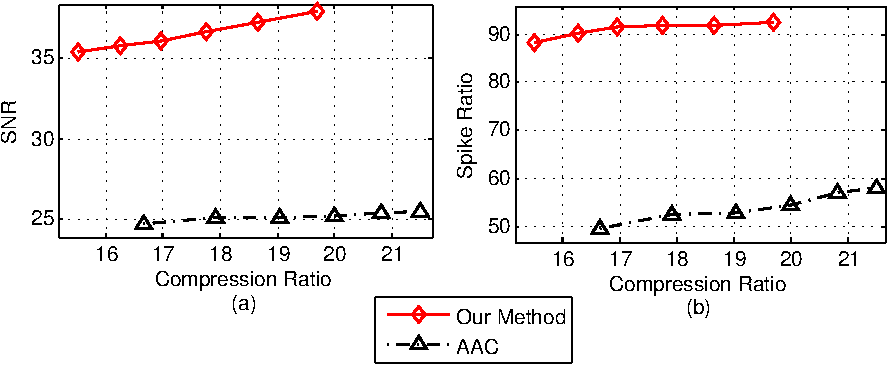
\includegraphics{Pictures/Compression/f13-crop.pdf}\\
  \caption{ 我们方法与音频编码方法压缩效果比较。 }\label{fig:Comparison-AAC and Ours}
\end{figure}


为了达到好的重构效果,我们对音频压缩选择高比特率,从 300kbps 到 600kbps。 

但是, 对于神经电信号,这两种方法的压缩效果并不理想。图中显示,在相同的压缩比下,我们的方法在两个信号保真度评判标准上都比AAC高, SNR超出AAC 46.4\%, Spike ratio超出AAC 80.4\%。 原因是音频压缩方法AAC在压缩过程中不关心哪部分对神经信号的处理比较重要。 实验结果也说明了神经电信号的信号特性有别于音频信号, 所以常规压缩方法不能很好地作用于神经电信号。 





\subsection{计算代价}
之前的小节描述了我们提出的算法在权衡Compression Ratio 和 重构误差时的有效性。 最后,我们讨论该算法的压缩效率。 一下结果是从我们在MATLAB上的实现中得来的统计结果。 初始化过程获取量化表, 哈夫曼码表和 无损压缩部分的分界线$B$ 速度为2.86Mb/s, 压缩过程为 0.13Mb/s, 解压速度为 0.14Mb/s。 如果用其他语言实现该算法压缩过程应该会得到更大提速。 




\section{结论}
本章提出了一个运动皮层神经电信号的压缩方法。 它在信号频谱采用提出的双阶编码方法进行信号压缩。 时序信号首先转换到频域, 然后通过一个幅值滤波器将信号分为 高幅值分量 和 低幅值分量, 然后分别对其进行编码。 为了压缩低幅值分量, 我们采用符号编码,对每个值只记录1bit的符号; 对于高幅值分量, 我们将其量化, 然后采用混合编码方法进行编码。 

之后, 我们将所提出的方法与其他压缩方法进行了比较。 可以看出, 在一定的Compression Ratio的情况下, 与其他方法相比, 我们的方法在重构效果(SNR 和 Spike Ratio)上都更胜一筹。 最终我们的压缩算法达到 17.7\% 的压缩比, SNR 为 36.6dB, 并保证91.9\%的 Spike 保真度。 该结果与其他神经信号压缩方法相比也很出众, 其他神经信号压缩方法只能使SNR达到 15-26dB, 压缩到元数据的1-20\%\cite{15,16,25}。 我们的算法在运动皮层(M1区)采集的神经电信号上进行了验证, 但是它也可以应用到其他神经信号上。 而且,如果考虑到其他信号的通道间相关性, 可以进一步提升压缩性能。 

而且, 基于统计结果而得的量化表,哈夫曼码表和其他参数可以根据信号被预先计算好。 我们的压缩框架原型成功地在猕猴运动皮层捕获信号上通过测试。 压缩效果比较理想, 只是有个缺陷, 本算法需要迭代求解, 因此比较耗时, 但由于压缩过程没有时序要求, 所以可在后期通过并行加速。












